\documentclass{beamer}
\usetheme{Boadilla}

\usepackage{amsmath}
\usepackage{amsfonts}
\usepackage{hyperref}

\usepackage{amsmath}
\DeclareMathOperator*{\argmax}{arg\,max}
\DeclareMathOperator*{\argmin}{arg\,min}

\title{Rényi Divergence Variational Inference}
\author{Kseniia Petrushina}
\institute{MIPT, 2023}


\begin{document}

\begin{frame}
    \titlepage
\end{frame}


\begin{frame}
    \tableofcontents
\end{frame}


\section{Motivation \& Background}
\begin{frame}{Motivation}
    \begin{block}{Main idea}
    Approximate inference is a crucial component of modern probabilistic machine learning, as it involves approximating posterior distributions and likelihood functions.

    The authors suggest combining existing methods into a unified framework.
    \end{block} 
\end{frame}


\begin{frame}{Background}
 \begin{block}{Variational inference}
    Posterior distribution
    \begin{equation}
        p(\boldsymbol{\theta}| \mathcal{D}, \varphi) = \dfrac{p(\boldsymbol{\theta}, \mathcal{D}| \varphi)}{p(\mathcal{D} | \varphi)}
    \end{equation}
    Variational lower-bound of $p(\mathcal{D}|\varphi)$
    \begin{equation}
        \mathcal{L}_{VI}(q; \mathcal{D}, \varphi) = \log{p (\mathcal{D}| \varphi)} - KL [q || p] = \mathbb{E}_q \Bigl[ \log{\dfrac{p(\boldsymbol{\theta}, \mathcal{D}| \varphi)}{q(\boldsymbol{\theta})}} \Bigr]
    \end{equation}
    \end{block}
    
    \begin{block}{Rényi’s \alpha-divergence}
    \begin{equation}
        D_\alpha [ p || q] = \dfrac{1}{\alpha - 1}\log \int p(\boldsymbol{\theta})^\alpha q(\boldsymbol{\theta})^{1-\alpha} d \boldsymbol{\theta}
    \end{equation} 

    \begin{enumerate}
            \item continuous and non-decreasing on $\alpha \in \{\alpha: |D_\alpha| < +\infty\}$
            \item for $\alpha \not \in \{0, 1\}, D_\alpha[p || q] = \dfrac{\alpha}{1 - \alpha } D_{1-\alpha}[p || q] \rightarrow D_\alpha[p || q] \le 0, \alpha <0$
        \end{enumerate}
        
    \end{block}
\end{frame}

\section{Theory}
\begin{frame}{Variational Rényi bound}
    \begin{block}{Definition}
    \begin{equation} \mathcal{L}_{\alpha}(q; \mathcal{D}, \varphi) = \log{p (\mathcal{D}| \varphi)} - D_\alpha [q || p] = \dfrac{1}{1-\alpha} \mathbb{E}_q \Bigl[ \log{ \Bigl( \dfrac{p(\boldsymbol{\theta}, \mathcal{D} | \varphi) }{q(\boldsymbol{\theta})} \Bigr)^{1-\alpha} } \Bigr]
    \end{equation} 

    \end{block}
    \begin{block}{Theorem 1}
    For all $\alpha_+ \in  (0, 1)$ and $\alpha_- < 0$
    \begin{equation}
        \mathcal{L}_{\alpha} (q; \mathcal{D}) = \lim\limits_{\alpha \to 1} \mathcal{L}_\alpha (q; \mathcal{D}) \le \mathcal{L}_{\alpha_+} (q; \mathcal{D}) \le \mathcal{L}_0 (q; \mathcal{D}) \le \mathcal{L}_{\alpha_-} (q; \mathcal{D})
    \end{equation} 
    \begin{equation}
        \mathcal{L}_0 (q; \mathcal{D}) = \log p(\mathcal{D}) \Leftrightarrow \text{supp}{(p(\boldsymbol{\theta} | \mathcal{D}))} \subseteq \text{supp}{(q(\boldsymbol{\theta}))} 
    \end{equation}
    \end{block}
    
\end{frame}


\begin{frame}{Variational Rényi bound}
    \begin{figure}
        \centering
        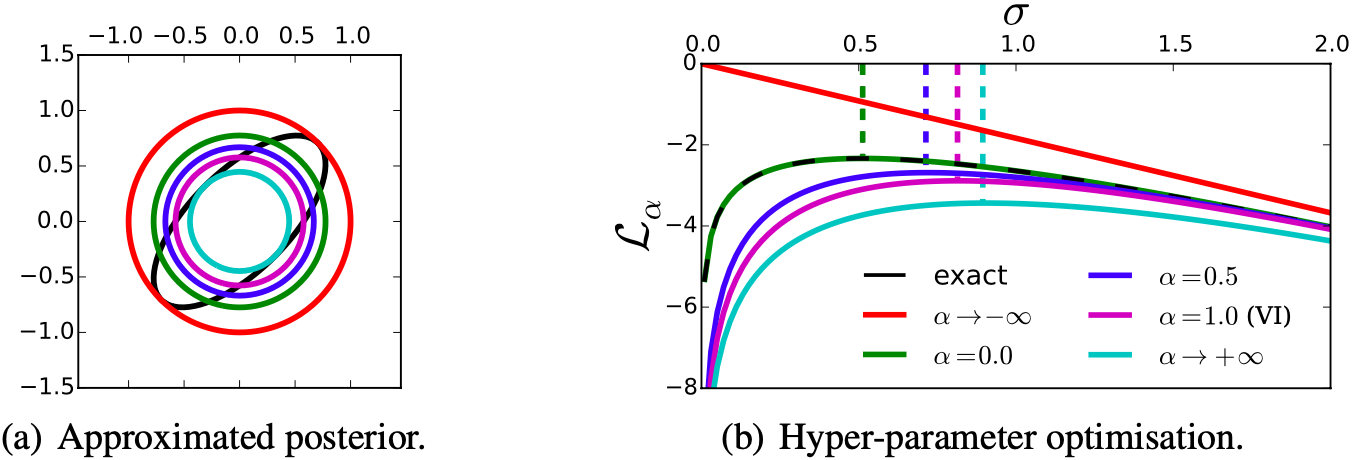
\includegraphics[scale=0.24]{normal.png}
        \caption{Mean-Field approximation for Bayesian linear regression.}
        \label{fig:enter-label}
    \end{figure}
\end{frame}

\begin{frame}{Monte Carlo approximation}
% \centering
\begin{block}{Approximation formula}
    \begin{equation}
        \hat{\mathcal{L}}_{\alpha, K} (q; \boldsymbol{x}) = \dfrac{1}{1-\alpha}  \log \dfrac1K \sum\limits_{k=1}^K \Bigl[ { \Bigl( \dfrac{p(\boldsymbol{\theta}_k, \textbf{x}) }{q(\boldsymbol{\theta}_k | \boldsymbol{x} )} \Bigr)^{1-\alpha} } \Bigr],
        \boldsymbol{\theta}_k \sim q(\boldsymbol{\theta} | \boldsymbol{x})
    \end{equation}

\end{block}

        \begin{figure}
        \centering
        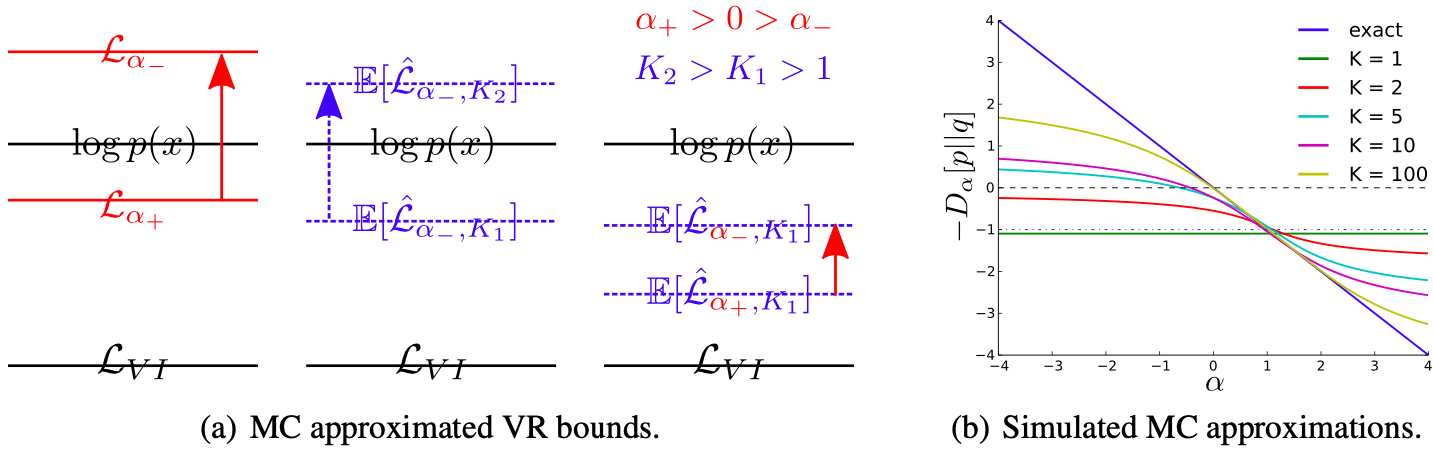
\includegraphics[scale=0.23]{mc.png}
        \caption{Monte Carlo approximation to the VR bound.}
        \label{fig:enter-label2}
    \end{figure}
\end{frame}

\section{Empirical results}
\begin{frame}{Bayesian neural network}
    \begin{figure}
        \centering
        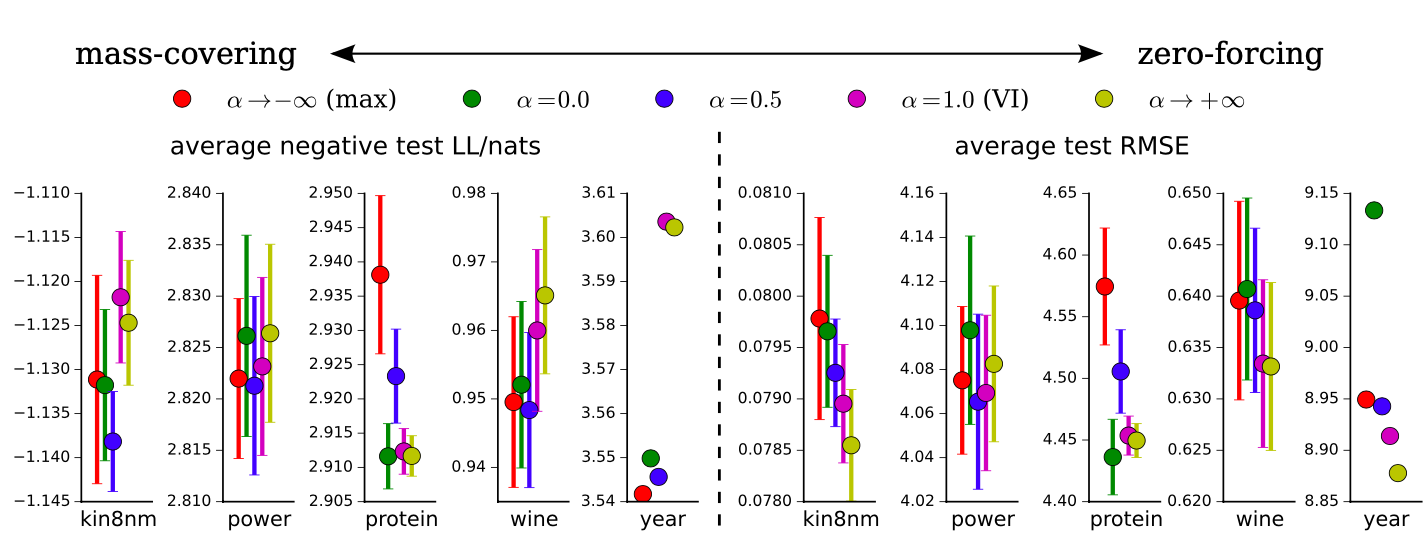
\includegraphics[scale=0.24]{bnn.png}
        \caption{Test LL and RMSE results for Bayesian neural network regression.}
        \label{fig:enter-label3}
    \end{figure}
\end{frame}

\begin{frame}{Variational auto-encoder}
    \begin{table}[]
        \centering
        \begin{tabular}{l c c c c}
        \hline
             \textbf{Dataset} & K & \textbf{VAE} & \textbf{IWAE} & \textbf{VR-max }\\
             \hline

                Frey Face & 5 &1322.96&\textbf{ 1380.30} & 1377.40\\
                (± std. err.) & & ±10.03 & \textbf{±4.60} & ±4.59 \\
                \hline
            Caltech 101  &5 &-119.69 &\textbf{-117.89} & -118.01 \\
                Silhouettes  & 50 & -119.61 &-117.21& \textbf{-117.10} \\
                \hline
                MNIST  &5& -86.47 & \textbf{-85.41} & -118.01  \\
                 &   50 &-86.35& \textbf{-84.80}& -117.10 \\
                 
                 \hline
                 OMNIGLOT &  5 &-107.62 &\textbf{-106.30} & -106.33\\
                  &50 &-107.80& \textbf{-104.68}&-105.05 \\
                 \hline
                
        \end{tabular}
        \caption{Average Test log-likelihood.}
        \label{tab:my_label}
    \end{table}
\end{frame}


\begin{frame}{Literature}
    \begin{enumerate}
        \item \textbf{Main article} \href{https://proceedings.neurips.cc/paper_files/paper/2016/file/7750ca3559e5b8e1f44210283368fc16-Paper.pdf}
        {Rényi Divergence Variational Inference}.
    \end{enumerate}
\end{frame}



\end{document}